 
\subsubsection{ Общие принципы и введение в алгоритм}

Имитация отжига — метод локального поиска, заимствующий аналогию из металлургии: при медленном охлаждении металла его атомы успевают занять состояние с минимальной энергией, тогда как быстрое охлаждение «замораживает» металл в случайном, не обязательно наилучшем состоянии. В применении к оптимизации это означает следующее: алгоритм работает с одним текущим решением и на каждом шаге пробует случайное небольшое изменение этого решения (один «ход»). Если изменение улучшает решение, оно принимается всегда. Если изменение ухудшает решение, оно всё равно может быть принято — но с вероятностью, которая убывает по мере того, как убывает управляющий параметр алгоритма, называемый температурой. На старте, при высокой температуре, алгоритм почти всегда соглашается на ухудшающие ходы, что позволяет ему свободно перемещаться по пространству решений и не застревать в первом найденном локальном оптимуме. По мере охлаждения вероятность принять ухудшение падает, и к концу работы алгоритм ведёт себя как обычный жадный локальный поиск, только уже отталкиваясь от гораздо более удачной стартовой точки, чем в начале.

При выборе инструмента для реализации имитации отжига изначально рассматривался готовый решатель scipy.optimize.dual_annealing — однако его применение к задаче расписания было признано нецелесообразным и впоследствии заменено самостоятельной реализацией. Причина в том, что dual_annealing, как и большинство готовых реализаций имитации отжига в общих научных библиотеках, спроектирован для задач с непрерывными переменными в заданных границах: представление решения в нём — это вектор вещественных чисел, а не дискретный набор категориальных решений (номер аудитории, идентификатор преподавателя). Применение такого решателя к дискретной задаче требовало бы искусственного округления вещественных координат до целочисленных индексов внутри функции оценки качества, что превращает функцию оценки в кусочно-постоянную и обесценивает встроенный в решатель механизм локальной градиентной доводки решения, рассчитанный на гладкие функции. Вместо этого был реализован классический дискретный вариант имитации отжига, работающий непосредственно с теми же дискретными ходами (изменение дня и пары занятия, замена аудитории, замена преподавателя, обмен временными слотами между двумя занятиями), что и в поиске с запретами, описанном в следующем разделе — но принципиально иначе использующий эти ходы: без памяти о предыдущих состояниях и с вероятностным, а не детерминированным критерием принятия.

\subsubsection{ Особенности реализации}

Каждая итерация алгоритма генерирует ровно один случайный ход и применяет его непосредственно к текущему расписанию, не создавая его копию — в отличие от поиска с запретами, где на каждой итерации оценивается целый пакет ходов-кандидатов. Это решение продиктовано тем, что имитация отжига обычно требует существенно большего числа итераций для полноценного прохождения цикла охлаждения, и копирование всего расписания на каждую (в большинстве случаев — отклонённую) попытку оказалось бы неоправданно расточительным. Вместо копирования реализован явный механизм отмены хода: каждая функция применения хода возвращает прежнее значение изменённого элемента расписания, и в случае отказа от хода это прежнее значение возвращается на место.

\captionof{listing}{Логика принятия и отклонения шага}
\begin{minted}{python}
delta = energy(candidate) - energy(current)
if delta <= 0 or random() < exp(-delta / temperature):
    accept_move()
else:
    revert_move()
temperature *= cooling_rate
\end{minted}

Отдельного внимания заслуживает то, что критерий принятия хода и критерий отбора лучшего из найденных решений за всю историю работы реализованы по-разному и намеренно не смешаны между собой. Для критерия принятия пара чисел «нарушения жёстких ограничений, штраф по мягким ограничениям» сводится к одному вещественному числу — иначе формула вероятности принятия, требующая единственного числового значения разницы энергий, была бы неприменима. Но при отборе лучшего решения за всю историю поиска используется точное сравнение исходной пары чисел без сведения к одному значению, поскольку именно так сохраняется строгий приоритет допустимости расписания над его мягким качеством.

\subsubsection{ Метрики

\paragraph {Динамика поиска}

Алгоритм демонстрирует выраженный стохастический характер сходимости. На ранних этапах поиска наблюдается значительный «шум» вследствие принятия решений об ухудшении целевой функции, что позволяет алгоритму покидать локальные оптимумы. По мере снижения температуры (остывания) график сходимости приобретает плавный нисходящий характер.

\begin{figure}[h]
    \centering
    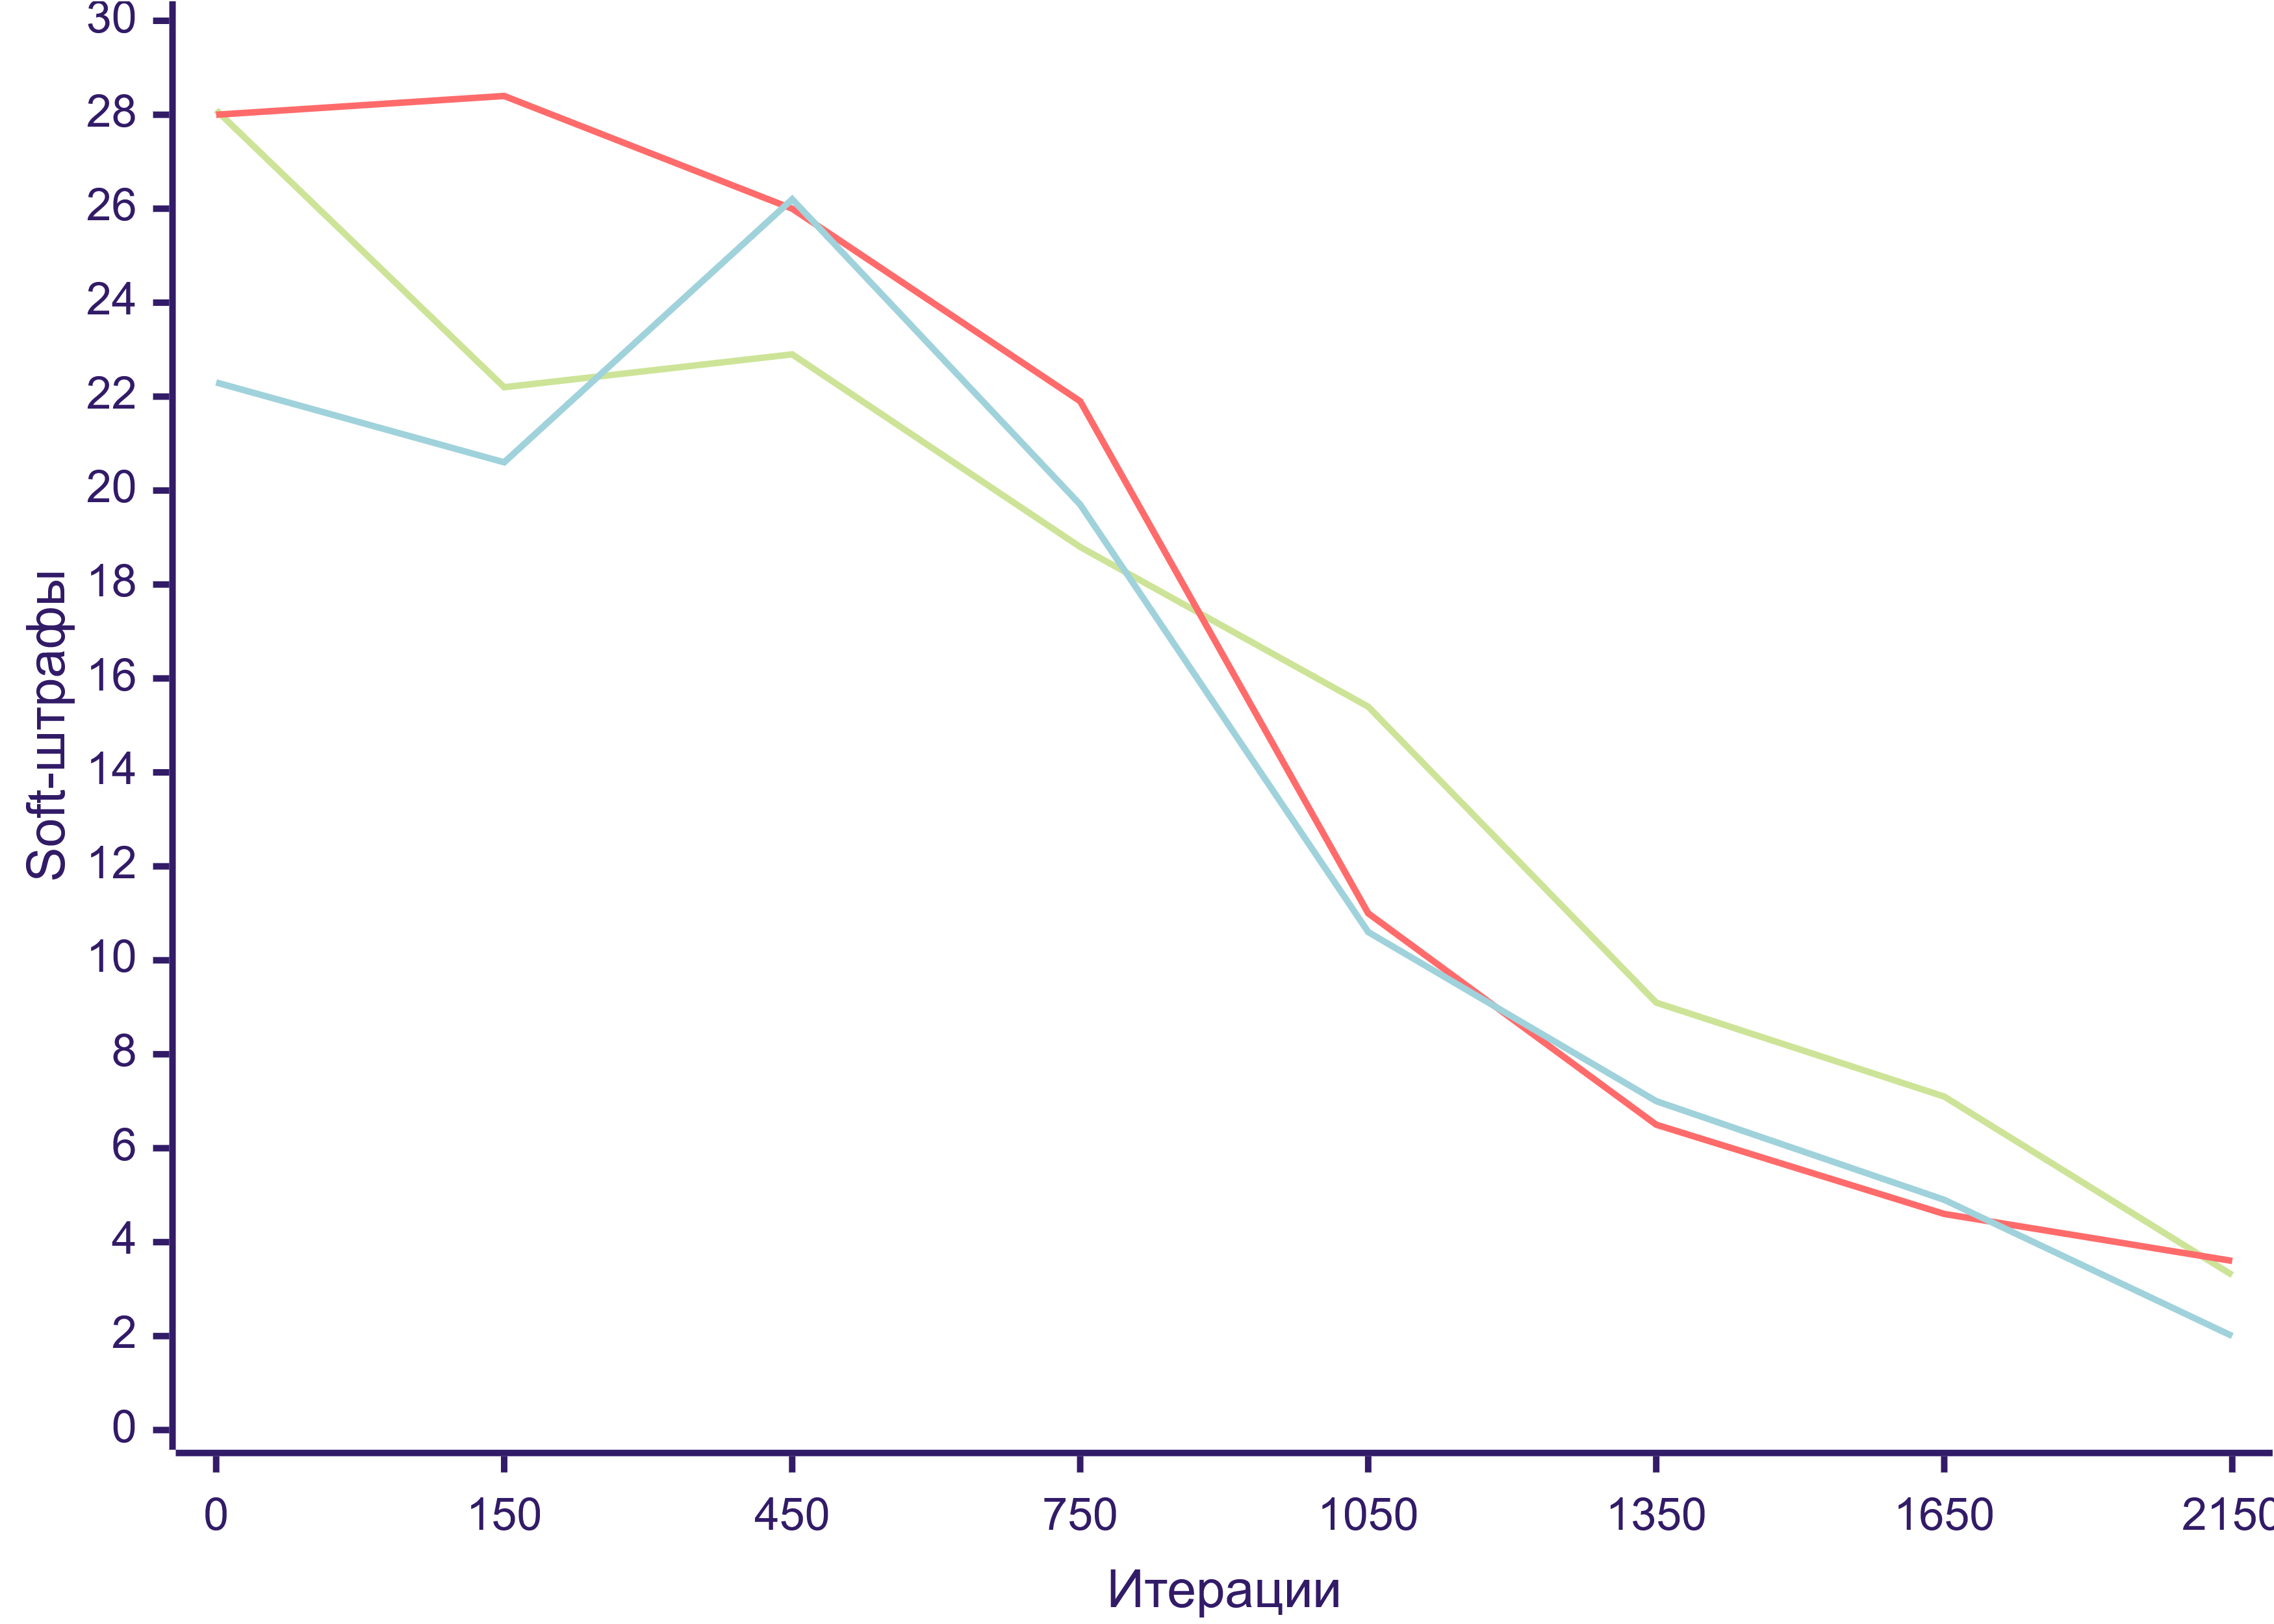
\includegraphics[width=0.8\textwidth]{images/SA Convergence.png}
    \caption{Сходимость SA: динамика soft-штрафов (medium)}
    \label{fig:SAConvergence}
\end{figure}

\paragraph {Анализ влияния гиперпараметров}

Экспериментально установлено, что эффективность метода имитации отжига критически зависит от стратегии охлаждения. При выборе высокой скорости охлаждения (cooling_rate = 0.999), мы наблюдаем прямую зависимость итогового качества решения от начальной температуры (initial_temperature). Увеличение начальной температуры до 200 позволяет алгоритму эффективнее преодолевать локальные оптимумы, обеспечивая снижение среднего штрафа с 0.95 до 0.84.

\begin{figure}[h]
    \centering
    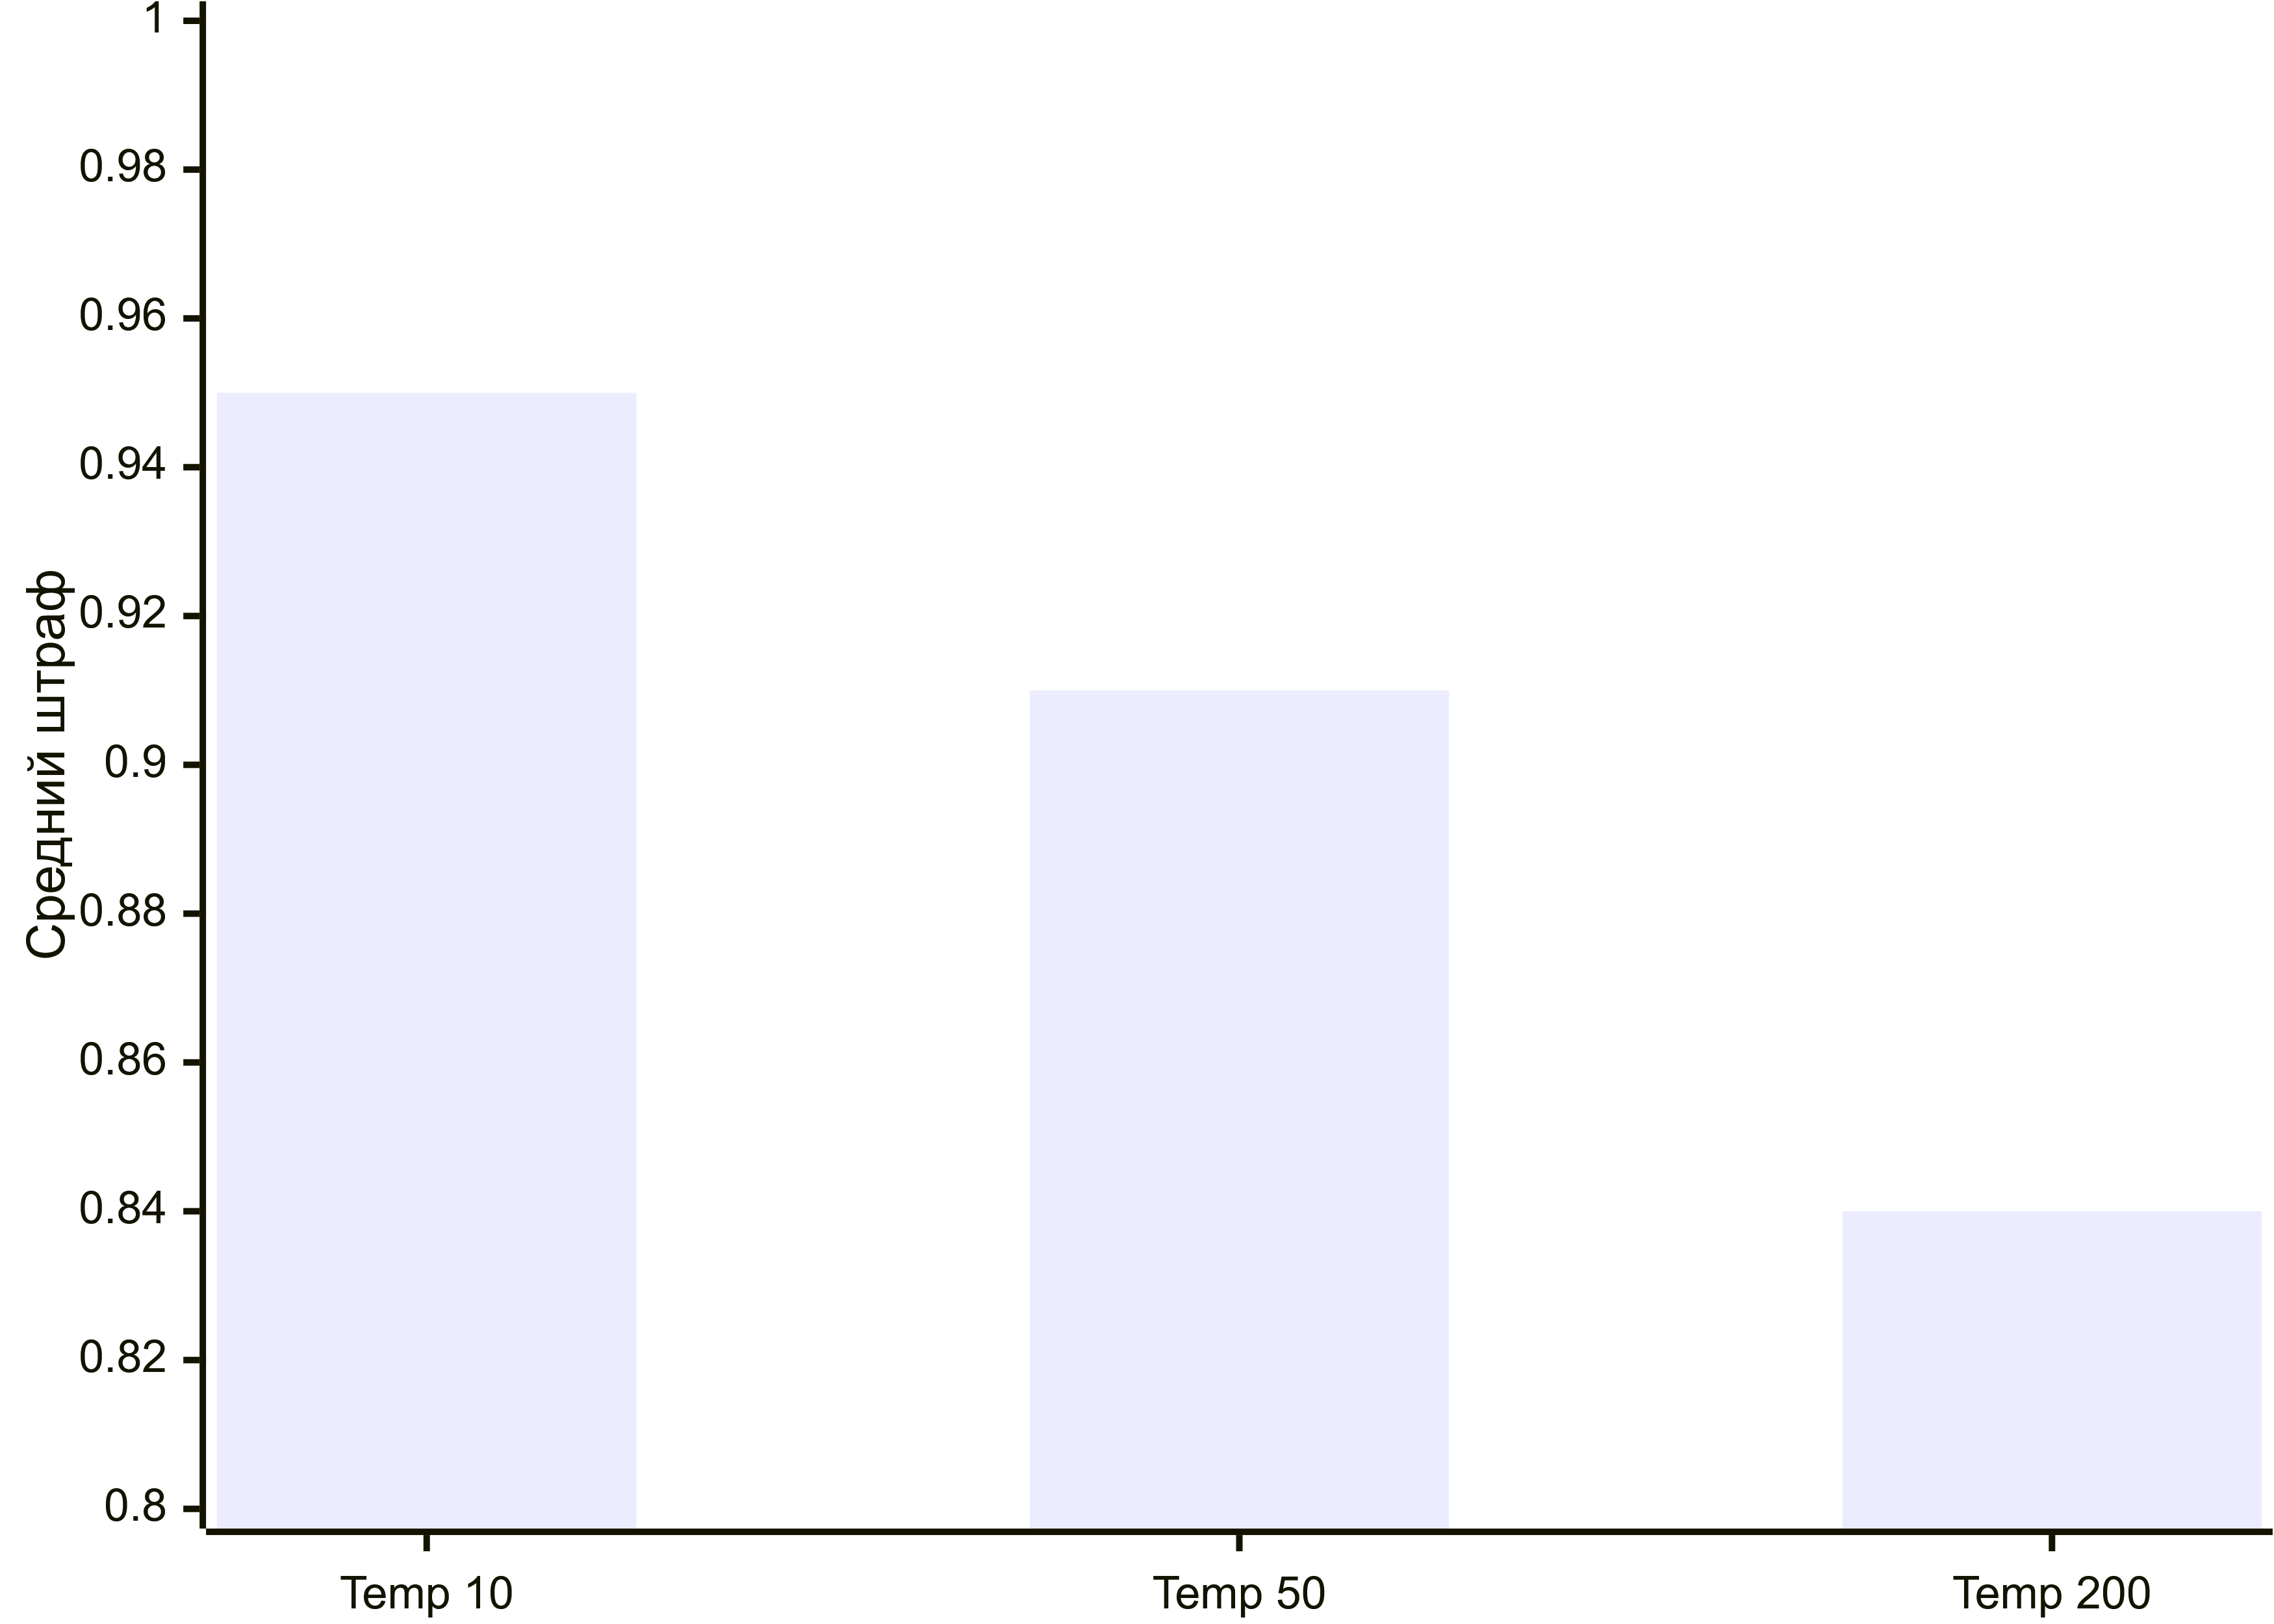
\includegraphics[width=0.8\textwidth]{images/SA Temperature.png}
    \caption{Зависимость штрафа от начальной температуры}
    \label{fig:SAtemperature}
\end{figure}

\subsubsection{ Проблемы, возникшие в процессе реализации}

В процессе анализа выбранных по умолчанию числовых параметров алгоритма была выявлена содержательная, хотя и не приводящая к видимому сбою, проблема масштаба. Коэффициент, с которым число нарушений жёстких ограничений входит в сводное числовое значение энергии, выбран заведомо большим по отношению к типичным значениям штрафа по мягким критериям — это сделано намеренно, чтобы любое ухудшение по жёстким ограничениям всегда расценивалось как существенно более плохое решение, чем любое ухудшение по мягким. Однако стартовое значение температуры было выбрано без учёта этого масштаба и оказалось на порядки меньше, чем типичная разница энергий при изменении числа жёстких нарушений на единицу. Это привело к тому, что вероятность принять ход, временно увеличивающий число жёстких нарушений ради последующего выхода из локального оптимума — то есть к самой сути метода имитации отжига, — оказывается на практике пренебрежимо малой: алгоритм фактически ведёт себя как обычный жадный локальный поиск по отношению к жёстким ограничениям, и только по отношению к мягким критериям действительно «отжигается» так, как это задумано методом. Эта проблема не была обнаружена через сбой или ошибку в логах, а была выявлена аналитически, при сопоставлении порядков величин двух связанных, но независимо выбранных числовых параметров — что говорит о необходимости содержательной, а не только эмпирической проверки гиперпараметров эвристических алгоритмов перед их использованием в сравнительном эксперименте.

Кроме того, имитация отжига в данной работе разделяла с генетическим алгоритмом и поиском с запретами общий дефект, связанный с ограничением на максимальный размер итогового расписания: контейнер для финального результата создавался с ограничением, равным вместимости учебной сетки, а не числу занятий в задаче, что на крупном наборе данных приводило к незаметному усечению расписания и, как следствие, к ложно оптимистичной оценке его допустимости. Дефект был обнаружен и устранён одинаковым образом во всех трёх затронутых реализациях.

\subsubsection{ Выводы по алгоритму}

Имитация отжига оказалась самым быстрым из четырёх реализованных алгоритмов при стабильно приемлемом качестве решения, уступающем поиску с запретами, но превосходящем генетический алгоритм. Это согласуется с тем, что метод работает с одним решением и одним недорогим по сравнению с популяционным подходом ходом за итерацию, при этом не тратя время на поддержание и пересчёт памяти о предыдущих состояниях, как это делает поиск с запретами. Вместе с тем выявленная проблема масштаба между коэффициентом штрафа за жёсткие нарушения и стартовой температурой показывает, что качество работы имитации отжига существенно зависит от тщательного согласования числовых параметров между собой, а не только от их отдельного разумного выбора.
